\documentclass[11pt,a4paper]{article}
\usepackage[spanish]{babel}
\usepackage[T1]{fontenc}
\usepackage[utf8]{inputenc}
\usepackage{lmodern}
\usepackage{geometry}
\usepackage{graphicx}
\usepackage{float}
\geometry{margin=2.5cm}
\setlength{\parindent}{0pt}
\setlength{\parskip}{0.65em}
\begin{document}
\begin{center}
{\Large \textbf{Optimización}}\\[0.25em]
{\large Hoja 1. Optimización en geometría}\\[0.45em]
\end{center}

\section*{Reflexiones y caminos mínimos}

\textbf{Reto 1.} En dos vértices opuestos de un cubo hay una mosca y una araña. ¿Qué camino tiene que seguir la araña por la superficie del cubo para llegar a la mosca lo más rápido posible? La mosca no se mueve.
\begin{center}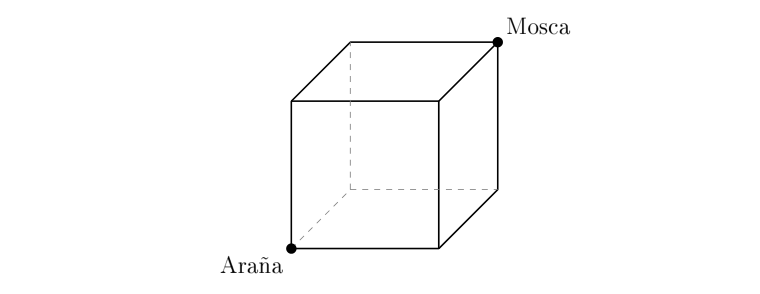
\includegraphics[width=0.65\linewidth]{figuras/reto1.png}\end{center}

\newpage

\textbf{Reto 3.} Dos pueblos están separados por dos ríos. ¿Dónde hay que construir los puentes (perpendiculares a las orillas) para que el camino de uno al otro sea más corto?
\begin{center}
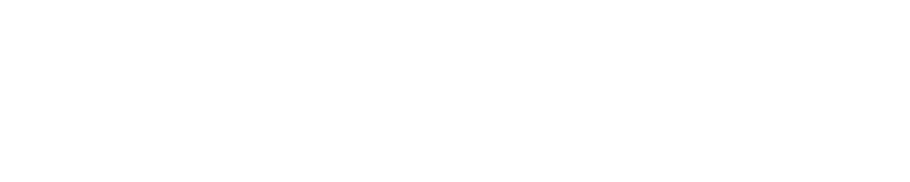
\includegraphics[width=0.78\linewidth]{figuras/reto3_parte1.png}\\[-1em]
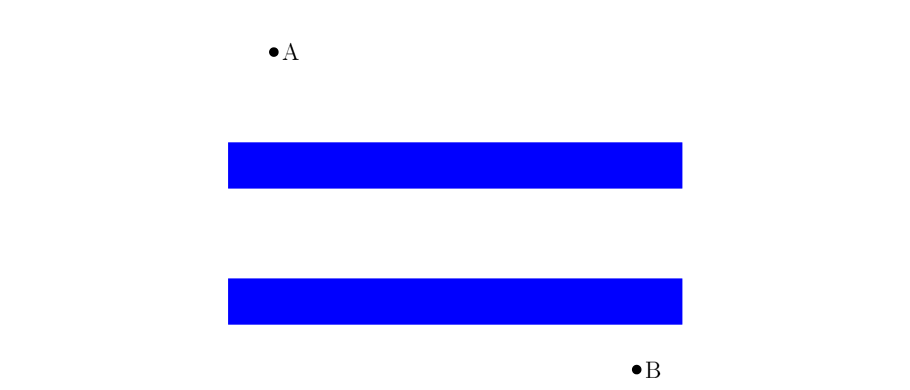
\includegraphics[width=0.78\linewidth]{figuras/reto3_parte2.png}
\end{center}

\newpage

\textbf{Reto 4.} En Manhattan, como bien se sabe, las calles forman una cuadrícula. Una empresa tiene sus sucursales en tres puntos de la ciudad, $A$, $B$ y $C$. La empresa quiere construir la sede en un punto de Manhattan donde la suma de distancias hasta las sucursales $A$, $B$ y $C$ sea mínima. Resuélvelo para ambos dibujos y para una posición arbitraria de los puntos $A$, $B$, $C$.
\begin{center}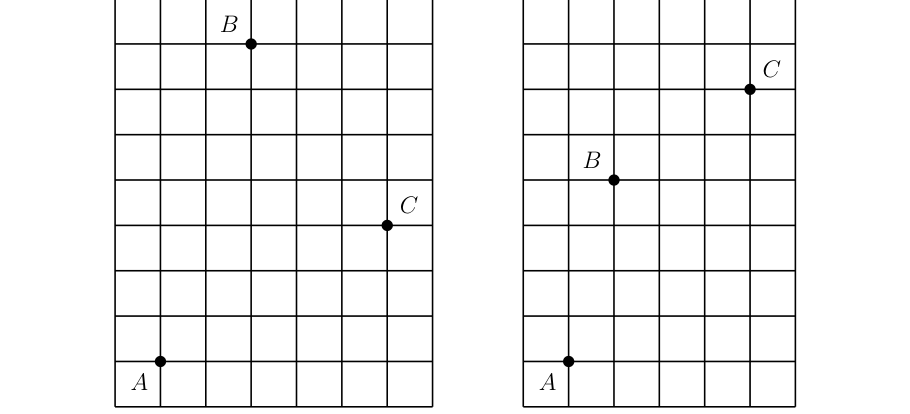
\includegraphics[width=0.92\linewidth]{figuras/reto4.png}\end{center}
¡Recuerda que en este caso sólo podemos movernos en horizontal o en vertical!

\newpage

\textbf{Reto 5.} Dentro de un ángulo se fijan dos puntos, $A$ y $B$. Salimos del punto $A$, llegamos a una semirrecta, luego nos dirigimos a la otra y, finalmente, llegamos al punto $B$. ¿Cómo minimizar este camino (rojo en el dibujo)?
\begin{center}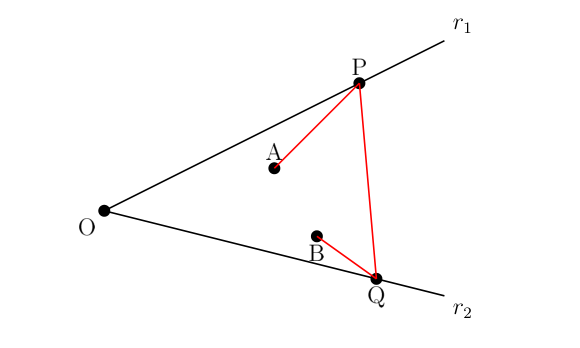
\includegraphics[width=0.60\linewidth]{figuras/reto5.png}\end{center}

\newpage

\textbf{Reto 6.} Dentro del ángulo agudo $BAC$ se da un punto $M$. Construir sobre los lados $BA$ y $AC$ los puntos $X$ e $Y$ de modo que el perímetro del triángulo $XYM$ sea mínimo.

\newpage

\textbf{Reto 7.} (2 puntos) Inscribe en un triángulo acutángulo dado $ABC$ un triángulo de perímetro mínimo.

\textbf{Pista.} Sea $A_1$ el vértice del triángulo buscado que pertenece al lado $BC$. Consideremos las imágenes de $A_1$ mediante las simetrías respecto a las rectas $AB$ y $AC$, y aplica el reto anterior.

\newpage

\section*{Puntos óptimos de un triángulo}

\textbf{Reto 8.} Desde un punto $M$ situado en el lado $AB$ de un triángulo acutángulo $ABC$ se bajan perpendiculares $MP$ y $MQ$ a los lados $BC$ y $AC$. ¿En qué posición del punto $M$ la longitud del segmento $PQ$ es mínima?

\newpage

\textbf{Reto 9.} Cuatro pueblos de la meseta deciden construir un hospital. ¿En qué lugar hay que construirlo para que la suma de las distancias hasta los cuatro pueblos sea mínima?

\textbf{Pista.} Estima por separado la suma de las distancias a cada pareja de pueblos opuestos.

\newpage

\section*{Tangencias, ángulos y una mosca en el espacio}

\textbf{Reto 13.} En un lado de un ángulo agudo se dan los puntos $A$ y $B$. Construir en el otro lado un punto $C$ desde el cual el segmento $AB$ se vea bajo el ángulo máximo.

\newpage

\textbf{Reto 14.} Dado el ángulo $\angle A$ y un punto $P$ en su interior, traza la recta que pase por $P$ y recorte del ángulo el triángulo de perímetro mínimo.

\newpage

\textbf{Reto 15.} Dado el ángulo $\angle XAY$ y un punto $O$ en su interior, traza por $O$ una recta que recorte del ángulo el triángulo de área mínima.

\textbf{Pista.} ¿Qué ocurre si el segmento de la recta que queda dentro del ángulo es dividido por el punto $O$ en dos partes iguales?
\end{document}
